\begin{frame}{Functional Sensitivity  \citep{gustafson:1996:local}}

\vspace{1em}

\begin{mdframed}[style=MyFrame]
\begin{center}
{\bf What about stick-breaking priors not in the Beta family?}
\end{center}
\end{mdframed}
\pause
Let $\p_0(\nu)$ be the stick-breaking prior used to compute $\etaopt$.
Suppose we wish to replace $\p_0(\nu)$ with another density, $\p_1(\nu)$. 

\pause
Define the ``perturbed'' prior as:
\begin{align*}
\p(\nu \vert \phi) \propto
\pbase(\nu)\exp(\phi(\nu))
\quad\textrm{with}\quad
\phi(\nu) = \log \p_1(\nu) - \log \p_0(\nu)
\end{align*}

\pause 

Then $\t \mapsto \p(\nu \vert \t \phi)$ 
parameterizes a path from $\pbase$ to $\palt$ for $\t \in [0,1]$.

\pause

\begin{figure}[!h]
\centering
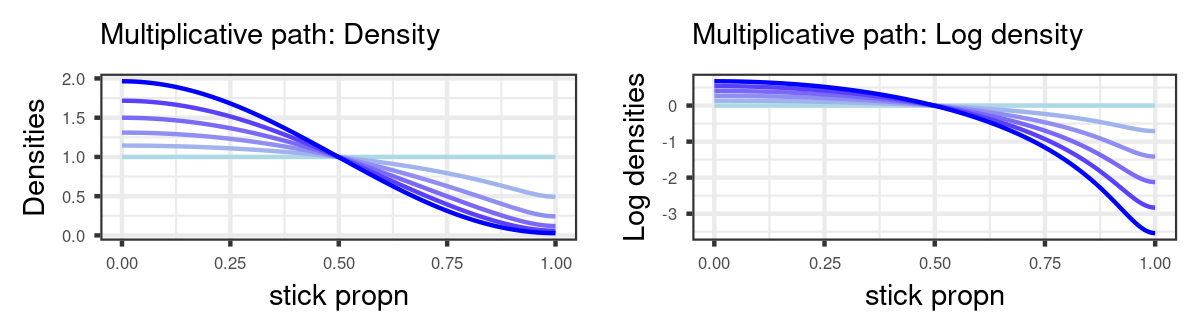
\includegraphics[width = 1.0\textwidth]{./figure/mult_path-1.png}
\setlength{\textfloatsep}{-10pt}
\end{figure}

\end{frame}





\begin{frame}{Functional Sensitivity  \citep{gustafson:1996:local}}

For any particular $\phi$, we can try to apply Theorem 1
to $\t \mapsto \p(\nu \vert \t \phi)$.  
          
\onslide<2->{
But it would be nice to safely search the space of functions $\phi$.
}

\onslide<3-> {
{\bf Questions:}
\begin{itemize}
    \item Can we specify a general condition on $\phi$ for
          Theorem 1 to apply?
    \item<4-> Is the derivative a good linear approximation for all
          such functions?
\end{itemize}
}

\begin{figure}[!h]
\centering
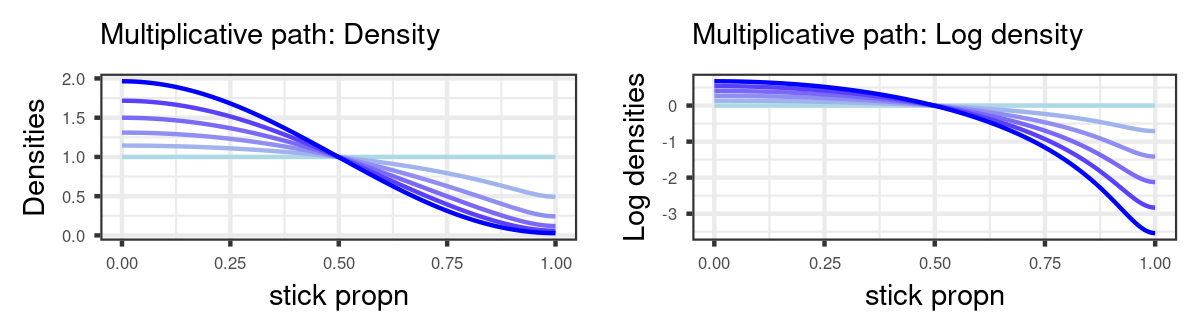
\includegraphics[width = 1.0\textwidth]{./figure/mult_path-1.png}
\setlength{\textfloatsep}{-10pt}
\end{figure}


\end{frame}









\begin{frame}{Functional Sensitivity: Differentiability}

% Let $\lp{\infty}$ denote the vector space of pointwise bounded functions
% measurable with respect to a measure dominating $\q(\nu \vert \eta)$ and $\pbase(\nu)$.
Let $\lp{\infty}$ denote the vector space of bounded, Lebesgue-measurable functions
with norm $\norminf{\phi} := \esssup_\nu \abs{\phi(\nu)}$.

\onslide<2->{
\textbf{Proposition.}

If $\phi \in \lp{\infty}$, then $\p(\nu \vert \phi)$ is a valid density
(positive and normalizable).
}

\onslide<3->{
\textbf{Theorem 2.}  (Validity of the derivative in $\lp{\infty}$.)
}

\onslide<4->{
If $\phi \in \lp{\infty}$, then the map $\t \mapsto \p(\nu \vert \t\phi)$
satisfies the conditions of Theorem 1, so $\t \mapsto \etaopt(\t \phi)$
is continuously differentiable.
}

\onslide<5->{
Further, the derivatives provides a uniformly
good linear approximation in an $\norminf{\cdot}$-neighborhood of the zero function.
%
In other words, the map $\phi \mapsto \etaopt(\phi)$ from
$\lp{\infty} \mapsto \mathbb{R}^D$ is {\em Fr{\'e}chet differentiable} at 
zero. \hfill $\square$
}

\onslide<6->{
{\bf Note:} Arguably, Fr{\'e}chet differentiability is a
minimal requirement for using the linear
approximation to safely search the space of functions.
}

\end{frame}





\begin{frame}{Functional Sensitivity: Influence Functions}

\textbf{Corollary of Theorem 2.} (Influence functions.)

Take a continuously differentiable quantity of
interest $g(\eta)$, e.g.
\begin{align*}
\g_{\textrm{cl}}(\eta) = \expect{\q_{\eta}} {\#\text{clusters}}
\end{align*}

\pause 
Let $S_g(\phi)$ be the \textit{local sensitivity} of $g$ in the direction $\phi$:
\begin{align*}
S_g(\phi) := \fracat{d g(\etaopt(\t \phi)) }{d\t}{\t=0}. 
\end{align*}

\pause

If $\norminf{\phi} < \infty$, the local sensitivity can be expressed as
an inner product between
an \textit{influence function} $\infl$ and the functional perturbation $\phi$:
\begin{align*}
S_g(\phi)   &=
    - \fracat{d g(\eta)}{d \eta^T}{\etaopt}
    \hessopt^{-1}
    \expect{\q_{\etaopt}}{
        \lqgrad{\nu \vert \etaopt}
        \phi(\nu)
    }
\\&=
\int \Psi(\nu) \phi(\nu) \;d\nu.
\end{align*}

\end{frame}








\begin{frame}{Iris Data: Influence Functions}
  \begin{figure}[!h]
    \centering
    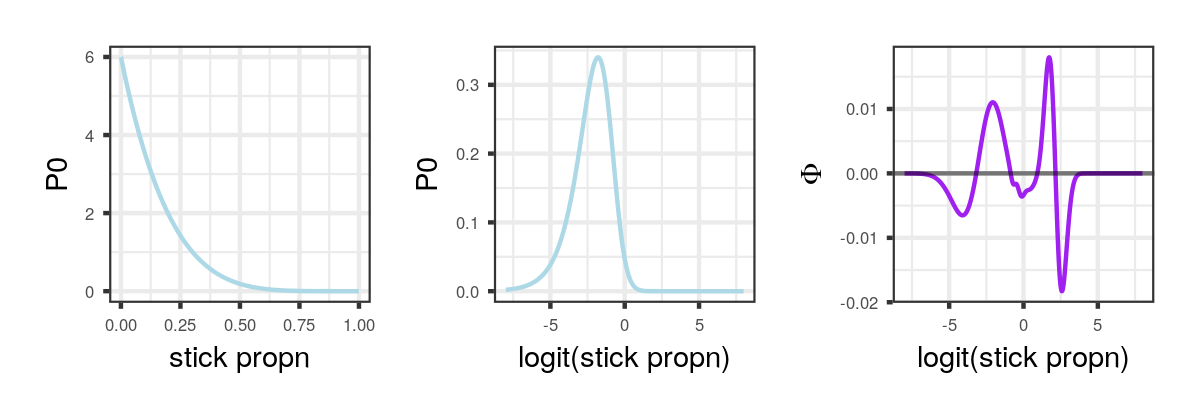
\includegraphics[width = \textwidth]{./figure/iris_infl-1.png}
    \caption*{The influence function for the number of clusters, $g_{\textrm{cl}}$.}
\end{figure}
\end{frame}

\begin{frame}{Iris Data: Functional Perturbations}
\begin{figure}[!h]
    \centering
    \only<1>{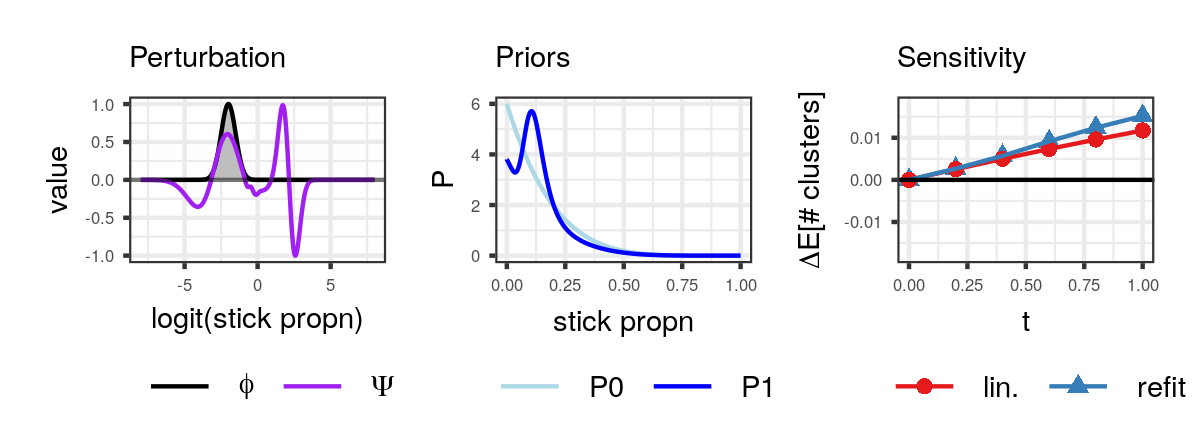
\includegraphics[width = \textwidth]{./figure/iris_fpertex-1.png}}
    \only<2>{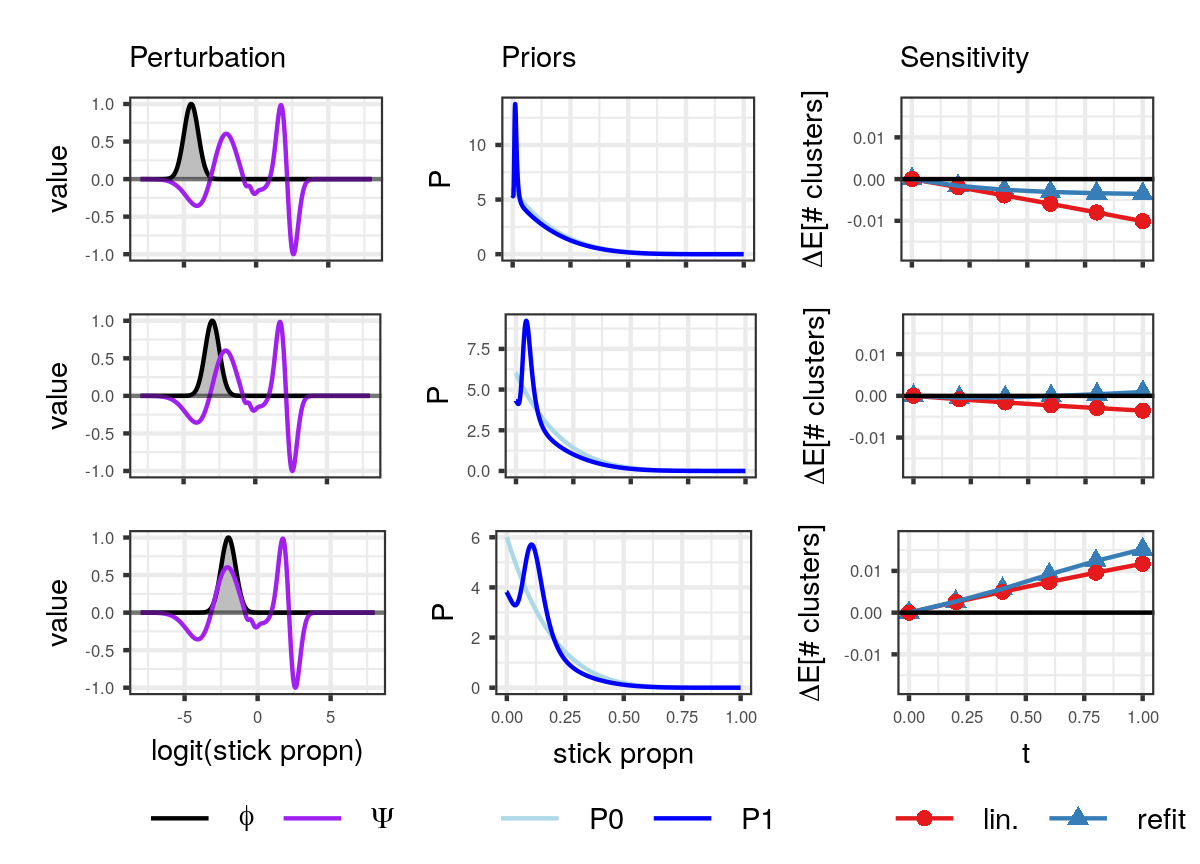
\includegraphics[width = \textwidth]{./figure/iris_fpertall-1.png}}
\end{figure}
\end{frame}






\begin{frame}{Functional Perturbations: Worst Case \citep{gustafson:1996:local}}

Which perturbation $\phi$ maximizes the sensitivity $S_g(\phi)$?

\pause
That is, can we find the {\bf worst-case} $\phi$ in the L-infinity ball of radius $\delta$,
%
\begin{align*}
  B_\delta := \{\phi : \|\phi\|_\infty < \delta\}?
\end{align*}

\vspace{-1em}

\pause
\begin{figure}[!h]
\centering
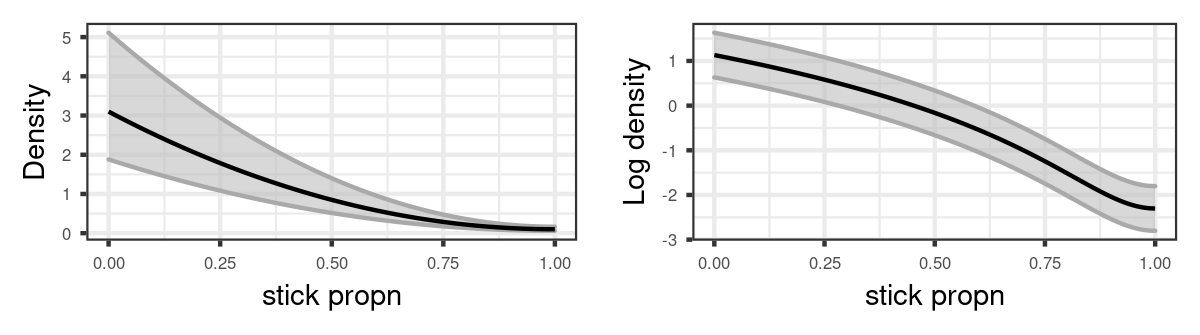
\includegraphics[width = 1.0\textwidth]{./figure/func_ball-1.png}
\setlength{\textfloatsep}{-10pt}
\end{figure}

\vspace{-2em}

\pause
Using the influence function and H{\"o}lder's inequality,
%
\begin{align*}
%
\sup_{\phi \in \ball_\delta} S_g(\phi) ={}&
\sup_{\phi \in \ball_\delta} \int \infl(\nu)\phi(\nu) d\nu
= \delta \int \abs{\infl(\nu)} d\nu, \textrm{ achieved at} \\
\phi^*(\nu) ={}& \delta \; \mathrm{sign}(\infl(\nu)).
%
\end{align*}
%
%achieved at $\phi^*(\nu) = \delta \; \mathrm{sign}(\infl(\nu))$.
%
\end{frame}






\begin{frame}{Iris Data: Worst-Case Perturbation}
  \begin{figure}[!h]
    \centering
    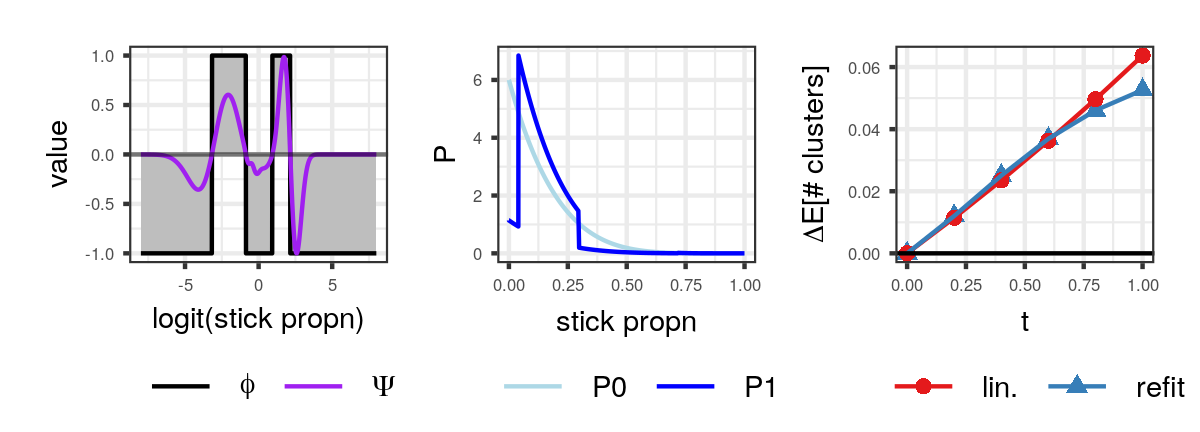
\includegraphics[width = \textwidth]{./figure/iris_worstcase-1.png}
\end{figure}

\pause

The worst-case prior may look unreasonable.  

But if the worst-case sensitivity is small, it is evidence of robustness.
\end{frame}